This section documents the integration of each unit into one algorithm that makes the application of the final system. The integration is validated according to the test specifications, section \ref{sec:testspec}, by feeding each output into the next unit and checking the results. 

\subsection{Implementation}
Each unit is integrated into one algorithm on behalf of the system specification in chapter \ref{ch3}. Algorithm \ref{alg:final} show the basic implementation of the final application. Note that each unit are imported as a function to be called and fed with their respective inputs in the final script, as showed in line 1.
\begin{algorithm}[H]
\caption{Final algorithm}
\begin{algorithmic}[1]
\State \textbf{import functions} FFT, Filter, STFT, Spectrogram, Peak\_dec  
\\
\Procedure{Import datafiles}{}
\State Return signal, freq \Comment{List of signal, sampling frequency}
\EndProcedure 
\\
\State $sampels = len(signal)$ 
\State $time   = sampels/float(freq)$
\State $cut1 = f_{c1}/freq$ \Comment {Filter specifications}
\State $cut2 = f_{c2}/freq$
\State $delta = \delta$
\State $tw = f_{tw}/freq$
\\
\Procedure  {Filtering of signal in frequency domain}{}
\State $SIGNAL = FFT(signal) $
\State $H = FFT(Filter(cut1,cut2,freq))$
\State $filt\_SIGNAL = SIGNAL \cdot H$
\State $filt\_signal = IFFT(filt\_SIGNAL)$ \Comment {Filtered signal in time domain} 
\EndProcedure 
\\
\Procedure {Generate spectrogram and detect peaks}{} 
\State $X = STFT(filt\_signal)$
\State $spec = Spectrogram(X,time,freq)$
\State $peaks = Peak\_dec(?,?)$
\EndProcedure
\\
\Procedure {Generate output}{}
\State $plot(spec)$ 
\State $plot(peaks)$
\EndProcedure
\end{algorithmic}
\label{alg:final}
\end{algorithm}      

\subsection{Integration test}
During the implementation the output of each step is printed and verified before implementing the next step. This is illustrated by figure \ref{fig:inte_validation}. The input signal consisting of a low E tone with noise in form of clapping hands.  

\begin{figure}[H]
\centering
\begin{subfigure}{0.49\textwidth}
\centering
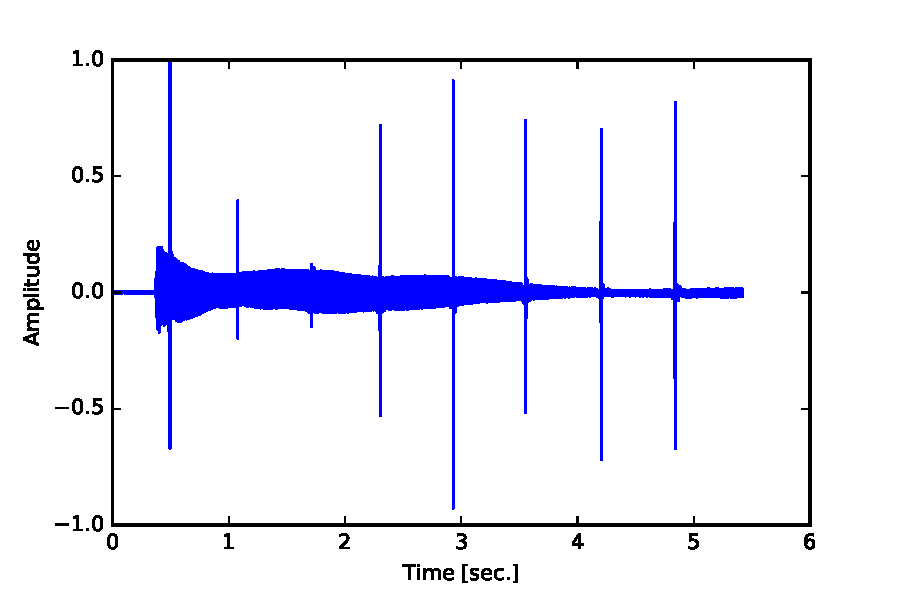
\includegraphics[width=\textwidth]{figures/validation/integration/signal.pdf}
\caption{Input signal with noise}
\label{fig:inte_signal}

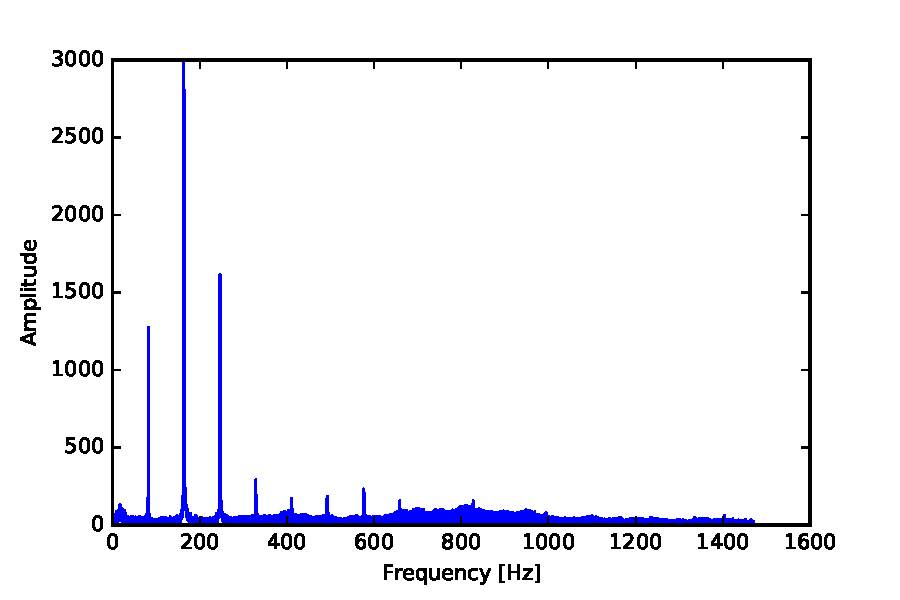
\includegraphics[width=\textwidth]{figures/validation/integration/f_signal.pdf}
\caption{Frequency spectrum of signal with noise}
\label{fig:inte_SIGNAL}
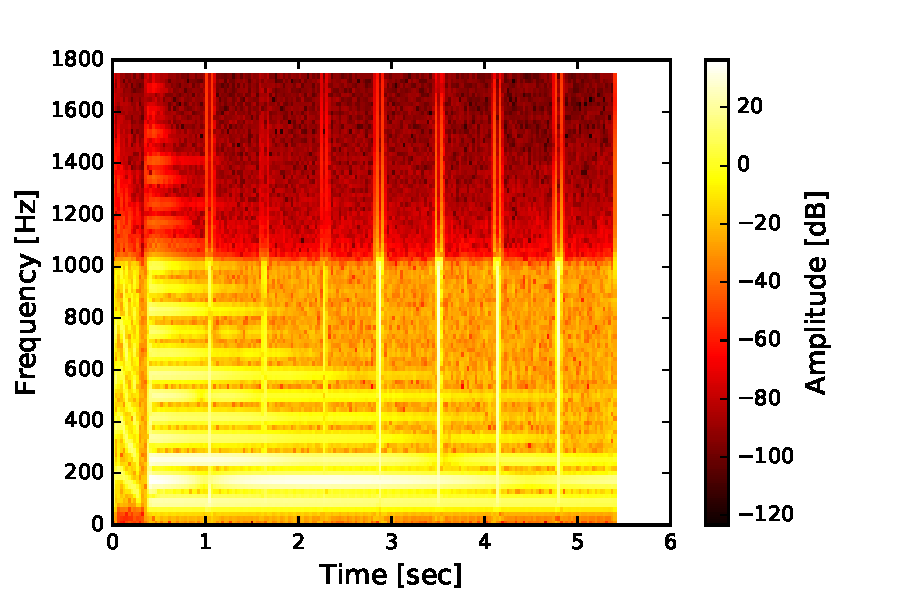
\includegraphics[width=\textwidth]{figures/validation/integration/spectrogram.pdf}
\caption{Spectrogram of filtered signal}
\label{fig:inte_spec}

\end{subfigure}
\begin{subfigure}{0.49\textwidth}
\centering

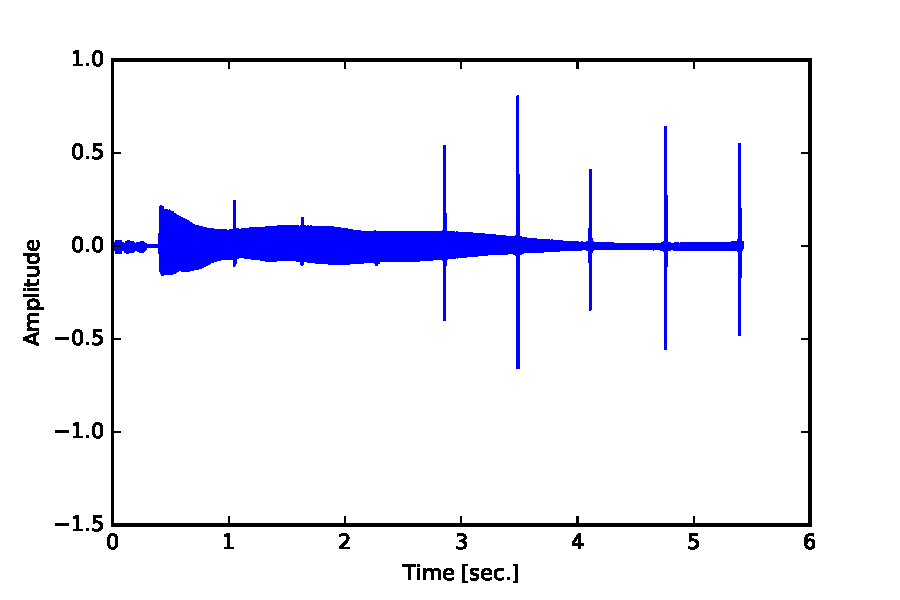
\includegraphics[width=\textwidth]{figures/validation/integration/signal_filt.pdf}
\caption{Filtered input signal with noise}
\label{fig:inte_signal_filt}
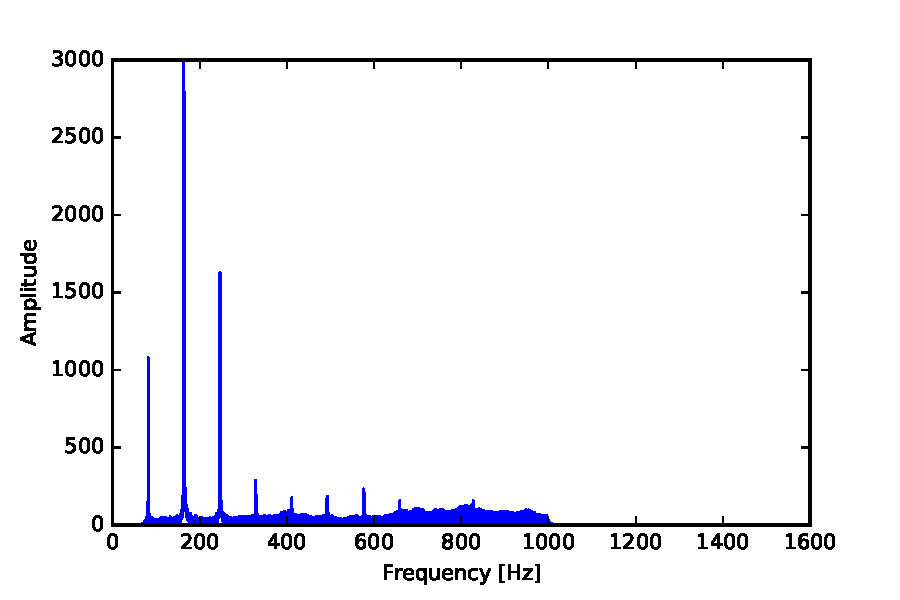
\includegraphics[width=\textwidth]{figures/validation/integration/f_signal_filt.pdf}
\caption{Frequency spectrum of filtered signal}
\label{fig:inte_SIGNAL_filt}
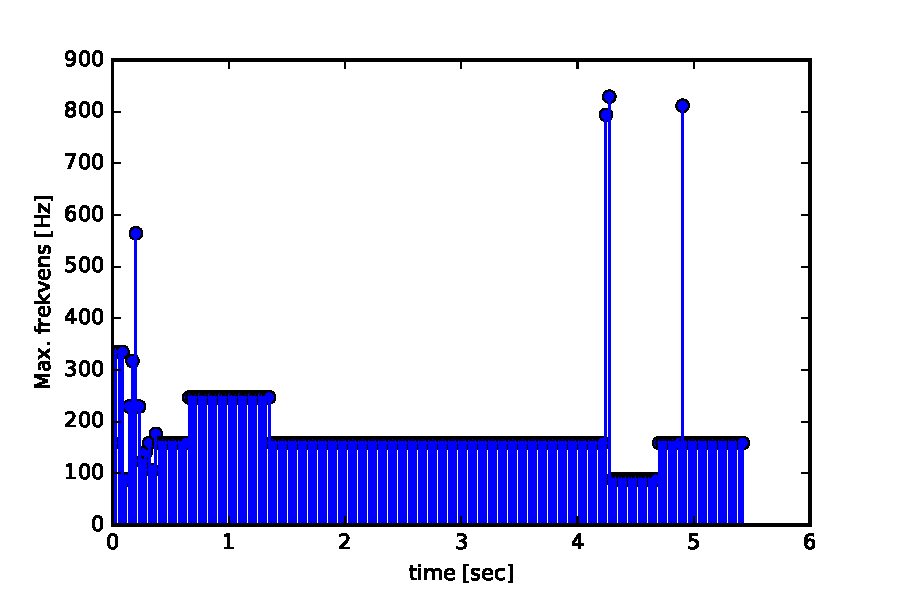
\includegraphics[width=\textwidth]{figures/validation/integration/peak_dec.pdf}
\caption{Maximum frequency over time}
\label{fig:inte_peak}

\end{subfigure}
\caption{Results of integration of each unit into one application }
\label{fig:inte_validation}
\end{figure}
Figure \ref{fig:inte_signal} and \ref{fig:inte_SIGNAL} show the input signal in time and frequency domain respectively. The FFT used is verified as the frequencies with highest amplitude is seen to correspond the known frequencies of an low E tone (82.41 [Hz]) and two corresponding overtones (164.82 [Hz] and 247.23[Hz])\trine{kan vi blot referere til frekvens analysen?}.Further noise appears similar to white noise across all frequencies.\\
Figure \ref{fig:inte_SIGNAL} and \ref{fig:inte_SIGNAL_filt} show the filtered signal in time and frequency domain respectively. Comparing this to the results of the unit test of the filter the result is the same hence the filtering is integrated as intended. Figure \ref{fig:inte_spec} show a valid spectrogram computed from the filtered signal. From the information in the spectrogram figure \ref{fig:inte_peak} show the frequency with the highest amplitude over time, which is seen to match the lightest point in the spectrogram.\\
\\
From this the implementation of each unit integrated into one script - forming the final application - is validated. \\
One can conclude that the final application is working as intended - corresponding to the level of the theory implemented. Whether this fulfil the practical purpose of the application when then input gets more complex is tested in the next section.              